\begin{name}
	{\tenchude}
	{\tendethi}
	{SỞ GDĐT TUYÊN QUANG}
	{\thoigian}
\end{name}

\caulc
\Opensolutionfile{ans}[Ans/TT-THPT-SGD-TuyenQuang-NH24-25]
%   \Opensolutionfile{ansbook}[Ansbook/TT-THPT-SGD-TuyenQuang-NH24-25-TN]%---Nên đặt tên theo bài
  \setcounter{ex}{0}
%%%==============Cau_EX1==============%%%
\begin{ex}%[Dự án C THPTQG 2025]%[ĐỖ CHÍ TÂM]%[2H1B1-1]
	Cho hình lập phương $ABCD.EFGH$ cạnh bằng $a$. Giá trị của $\vec{AC}\cdot\vec{EG}$ bằng
	\choice
	{$-a^2$}
	{$a^2$}
	{$-2a^2$}
	{\True$2a^2$}
	\loigiai{
		Ta có hình lập phương $ABCD.EFGH\Rightarrow \vec{AC}=\vec{EG}\Rightarrow \vec{AC}\cdot\vec{EG}=\vec{AC}\cdot\vec{AC}=AC^2$.\\
		Vì tam giác $ABC$ vuông tại $B$ nên $AC^2=BA^2+BC^2=a^2+a^2=2a^2$.
	}
\end{ex}
%%%==============HetCau_EX1==============%%%
%%%==============Cau_EX2==============%%%
\begin{ex}%[Dự án C THPTQG 2025]%[ĐỖ CHÍ TÂM]%[1D6N4-2]
	Tập nghiệm $S$ của phương trình $2^{x^2+7x+10}=1$ là 
	\choice
	{$S=\{2; 5\}$}
	{\True $\{-5; -2\}$}
	{$S=\{-5; 2\}$}
	{S=$\left\{\dfrac{-7-\sqrt{13}}{2}; \dfrac{-7+\sqrt{13}}{2}\right\}$}
	\loigiai{
		Ta có $2^{x^2+7x+10}=1\Rightarrow 2^{x^2+7x+10}=2^0\Rightarrow x^2+7x+10=0\Rightarrow x=-5\text{ hoặc }x=-2$
	}
\end{ex}
%%%==============HetCau_EX2==============%%%
%%%==============Cau_EX3==============%%%
\begin{ex} %[Dự án C THPTQG 2025]%[ĐỖ CHÍ TÂM]%[2D1Y2-2]
	\immini[thm]{
	Cho hàm số $y=f(x)$ có bảng biến thiên như hình vẽ. Tọa độ điểm cực đại của đồ thị hàm số là
	\choice
	{$(0; 2)$}
	{\True $(-2; 0)$}
	{$(0; -2)$}
	{$(2; 0)$}
	}{
	 
\begin{tikzpicture}
	 	\tkzTabInit[nocadre=true,lgt=1.2,espcl=2.5,deltacl=0.6]
	 	{$x$ /0.6,$f'(x)$ /0.6,$f(x)$ /2}
	 	{$-\infty$,$0$,$3$,$+\infty$}
	 	\tkzTabLine{,+,$0$,-,$0$,+,}
	 	\tkzTabVar{-/$-\infty$, +/$2$,-/$-4$,+/$+\infty$}
	 \end{tikzpicture}}
	\loigiai{	
		Ta thấy tại điểm $x = 0$ thì $f'(x)$ đổi dấu từ dương sang âm. Do đó điểm cực đại của đồ thị hàm số là $(0;2)$.
		
	}
\end{ex}
%%%==============HetCau_EX3==============%%%
%%%==============Cau_EX4==============%%%
\begin{ex}%[Dự án C THPTQG 2025]%[ĐỖ CHÍ TÂM]%[2H3Y1-1]
	Trong không gian với hệ trục tọa độ Oxyz , cho $2$ điểm $A (1; -2; -3)$ và $B ( 7 ; -14 ; 11 )$. Tọa độ trung điểm của đoạn thẳng $AB$ là
	\choice
	{$(-4; 8; -4)$}
	{\True $(4; -8; 4)$}
	{$(3; -6; 7)$}
	{$(-3; 6; -7)$}
	\loigiai{
		Gọi $M(x_M; y_M; z_M)$ là trung điểm của đoạn thẳng $AB$, ta có $$\heva{&x_M=\dfrac{x_A+x_B}{2}=\dfrac{1+7}{2}=4\\&y_M=\dfrac{y_A+y_B}{2}=\dfrac{-2-14}{2}=-8\\&z_M=\dfrac{z_A+z_B}{2}=\dfrac{-3+11}{2}=4.}$$
		Vậy $M(4; -8; 4)$.
	}
\end{ex}
%%%==============HetCau_EX4==============%%%
%%%==============Cau_EX5==============%%%
\begin{ex}%[Dự án C THPTQG 2025]%[ĐỖ CHÍ TÂM]%[1D2N2-4]
	Cho cấp số cộng $(u_n)$ có $u_1=1$ và công sai $d=3$. Số hạng $u_3$ của cấp số cộng là
	\choice
	{$10$}{\True $7$}{$9$}{$4$}
	\loigiai{
		Ta có $u_3=u_1+2d=1+2\cdot 3=7$.
	}
\end{ex}
%%%==============HetCau_EX5==============%%%
%%%==============Cau_EX6==============%%%
\begin{ex}%[Dự án C THPTQG 2025]%[ĐỖ CHÍ TÂM]%[2D1Y5-3]
	\immini{Cho hàm số $y=\dfrac{ax+b}{cx+d}$ có đồ thị như hình vẽ bên. Tọa độ giao điểm của đồ thị hàm số đã cho với trục hoành là
	\choice
	{$(0; 2)$}{$(-2; 0)$}{$(0; -2)$}{\True $(2; 0)$}}{
		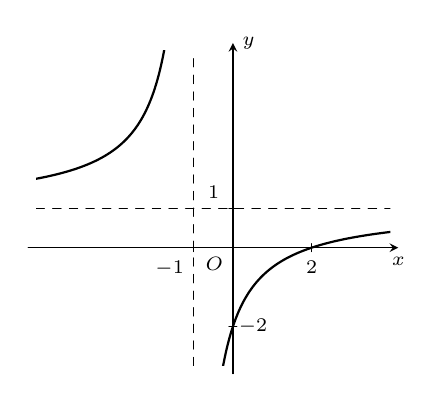
\begin{tikzpicture}[scale=0.5, line join=round, line cap=round, >=stealth,font=\scriptsize]
			\tikzset{every node/.style={scale=1}}
			\def\xmin{-5}\def\xmax{4}\def\ymin{-3}\def\ymax{5}
			\draw[->] (\xmin-0.2,0)--(\xmax+0.2,0) node[below]{$x$};
			\draw[->] (0,\ymin-0.2)--(0,\ymax+0.2) node[right]{$y$};
			\draw (0,0) node[below left]{$O$};
			\foreach \x in {-1}\draw (\x,0.1)--(\x,-0.1) node[below left]{$\x$};
			\foreach \x in {2}\draw (\x,0.1)--(\x,-0.1) node[below]{$\x$};
			\foreach \y in {1}\draw (0.1,\y)--(-0.1,\y) node[above left]{$\y$};
			\foreach \y in {-2}\draw (0.1,\y)--(-0.1,\y) node[right]{$\y$};
			\clip (\xmin,\ymin) rectangle (\xmax,\ymax);
			\draw[dashed] (\xmin,1.0)--(\xmax,1.0);
			\draw[dashed] (-1.0,\ymin)--(-1.0,\ymax);
			\draw[thick,smooth,samples=200,domain=\xmin:-1.1] plot (\x,{(1*(\x)+-2)/(1*(\x)+1)});
			\draw[thick,smooth,samples=200,domain=-0.9:\xmax] plot (\x,{(1*(\x)+-2)/(1*(\x)+1)});
		\end{tikzpicture}
	}
	\loigiai{
		Từ hình vẽ, ta suy ra đồ thị hàm số đã cho cắt trục hoành tại điểm $(2; 0)$.
	}
\end{ex}
%%%==============HetCau_EX6==============%%%
%%%==============Cau_EX7==============%%%
\begin{ex}%[Dự án C THPTQG 2025]%[ĐỖ CHÍ TÂM]%[2H3Y2-5]
	Trong không gian với hệ trục tọa độ $Oxyz$, cho hai véc-tơ $\vec u=(-1; 1; 0)$, $\vec v=(0; -1; 0)$. Góc giữa hai véc-tơ đã cho bằng
	\choice
	{$120^\circ$}{$60^\circ$}{\True $135^\circ$}{$45^\circ$}
	\loigiai{
		Ta có $$\cos(\vec u, \vec v)=\dfrac{\vec u\cdot\vec v}{|\vec u|\cdot|\vec v|}=\dfrac{-1\cdot 0+1\cdot(-1)+0\cdot 0}{\sqrt{(-1)^2+1^2+0^2}\sqrt{0^2+(-1)^2+0^2}}=-\dfrac{\sqrt2}{2}\Rightarrow(\vec u, \vec v)=135^\circ.
		$$
	}
\end{ex}
%%%==============HetCau_EX7==============%%%\\
%%%==============Cau_EX8==============%%%
\begin{ex}%[Dự án C THPTQG 2025]%[ĐỖ CHÍ TÂM]%[1D5H2-3]
	Kết quả thống kê chiều cao (đơn vị cm) của các bạn học sinh nữ lớp 12A ở bảng sau	
	\begin{center}
		\begin{tabular}{|c|c|c|c|c|c|}
			\hline
			Chiều cao (cm) & $[155; 160)$ & $[160; 165)$ & $[165; 170)$ & $[170; 175)$ & $[175; 180)$ \\
			\hline
			Số học sinh & $5$ & $9$ & $8$ & $2$ & $1$ \\
			\hline
		\end{tabular}
	\end{center}	
	Tứ phân vị thứ ba của mẫu số liệu ghép nhóm về chiều cao của học sinh nữ lớp 12A (làm tròn đến chữ số thập phân thứ hai) bằng
	\choice
	{$160{,}69$}{$168{,}59$}{$166{,}24$}{\True $167{,}97$}
	\loigiai{
		Ta có
		\begin{itemize}
			\item $n=5+9+8+2+1=25$.
			\item $\dfrac{3n}{4}=\dfrac{3\cdot 25}{4}=18{,}75$.
		\end{itemize}
		Vì $5+9<18{,}75<5+9+8$ nên $Q_3\in[165; 170)$.\\
		Suy ra $Q_3=165+\dfrac{18{,}75-(5+9)}{8}\cdot(170-165)\approx 167{,}97$.
		
	}
\end{ex}
%%%==============HetCau_EX8==============%%%
%%%==============Cau_EX9==============%%%
\begin{ex}%[Dự án C THPTQG 2025]%[ĐỖ CHÍ TÂM]%[1D6H4-3]
	Tập nghiệm $S$ của bất phương trình $\log_2(2x-1)\ge3$ là
	\choice
	{$\left[\dfrac52; +\infty\right)$}{\True $\left[\dfrac92; +\infty\right)$}{$\left(\dfrac72; +\infty\right)$}{$\left[\dfrac72; +\infty\right)$}
	\loigiai{
		Điều kiện xác định: $2x-1>0\Leftrightarrow x>\dfrac12$.\\
		Ta có $\log_2(2x-1)\ge 3\Leftrightarrow 2x-1\ge2^3\Leftrightarrow x\ge\dfrac92$.\\
		Kết hợp với điều kiện xác định, tập nghiệm bất phương trình là $S=\left[\dfrac92; +\infty\right)$.
	}
\end{ex}
%%%==============HetCau_EX9==============%%%
%%%==============Cau_EX10==============%%%
\begin{ex}%[Dự án C THPTQG 2025]%[ĐỖ CHÍ TÂM]%[2D1B1-2]
	\immini{Cho hàm số $y=ax^3+bx^2+cx+d$ ($a\ne0$) có đồ thị như hình vẽ bên. Hàm số đã cho nghịch biến trong khoảng nào sau đây?
	\choice
	{$(-\infty; -1)$ và $(1; +\infty)$}{$(0; +\infty)$}{$(-\infty; 0)$}{\True $(-1; 1)$}}{
		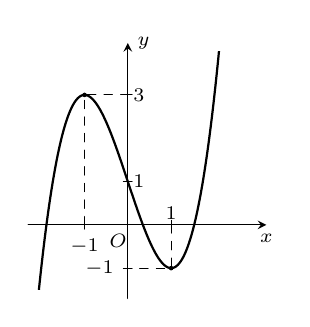
\begin{tikzpicture}[scale=0.55, line join=round, line cap=round, >=stealth,font=\scriptsize]
			\tikzset{every node/.style={scale=1}}
			\def\xmin{-2.1}\def\xmax{3}\def\ymin{-1.5}\def\ymax{4}
			\draw[->] (\xmin-0.2,0)--(\xmax+0.2,0) node[below]{$x$};
			\draw[->] (0,\ymin-0.2)--(0,\ymax+0.2) node[right]{$y$};
			\draw (0.2,0) node[below left]{$O$};
			\foreach \x in {-1}\draw (\x,0.1)--(\x,-0.1) node[below]{$\x$};
			\foreach \x in {1}\draw (\x,0.1)--(\x,-0.1) node[above]{$\x$};
			\foreach \y in {-1}\draw (0.1,\y)--(-0.1,\y) node[left]{$\y$};
			\foreach \y in {1,3}\draw (0.1,\y)--(-0.1,\y) node[right]{$\y$};
			\clip (\xmin,\ymin) rectangle (\xmax,\ymax);
			\draw[thick,smooth,samples=200,domain=\xmin:\xmax] plot (\x,{1*((\x)^3)+0*((\x)^2)+-3*(\x)+1});
			\draw[dashed] (-1,0)--(-1,3)--(0,3);\fill (-1,3)circle(1.5pt);
			\draw[dashed] (1,0)--(1,-1)--(0,-1);\fill (1,-1)circle(1.5pt);
		\end{tikzpicture}
	}
	\loigiai{
	Dựa vào đồ thị hàm số, ta suy ra hàm số đã cho nghịch biến trong khoảng $(-1; 1)$.}
\end{ex}
%%%==============HetCau_EX10==============%%%
%%%==============Cau_EX11==============%%%
\begin{ex}%[Dự án C THPTQG 2025]%[ĐỖ CHÍ TÂM]%[2D1Y4-1]
	\immini{Cho hàm số $y=f(x)$ có bảng biến thiên như hình vẽ bên. Đường tiệm cận ngang của đồ thị hàm số đã cho là
	\choice
	{$y=1$}{\True $y=2$}{$x=1$}{$x=2$}}{
		
\begin{tikzpicture}[font=\scriptsize,scale=0.65]
			\tkzTabInit[nocadre=false,lgt=1.2,espcl=2.5,deltacl=0.6]
			{$x$/1,$f'(x)$/1,$f(x)$/2}{$-\infty$,$1$,$+\infty$}
			\tkzTabLine{,-,d,-,}
			\tkzTabVar{+/$2$,-D+/$-\infty$/$+\infty$,-/$2$}
		\end{tikzpicture}
		
	}
	\loigiai{
		Từ bảng biến thiên, ta có $\lim\limits_{x\to-\infty}y=2$ và $\lim\limits_{x\to+\infty}y=2$.\\
		Suy ra đồ thị hàm số có đường tiệm cận ngang là $y=2$.
	}
\end{ex}
%%%==============HetCau_EX11==============%%%
%%%==============Cau_EX12==============%%%
\begin{ex}%[Dự án C THPTQG 2025]%[ĐỖ CHÍ TÂM]%[1H8H6-1]
	\immini{Cho hình chóp $S.ABCD$ có đáy là hình chữ nhật, $AB=a\sqrt3$, $SA\perp(ABCD)$ và $SB=2a$ (minh họa như hình bên). Góc giữa $SB$ và mặt phẳng $(ABCD)$ bằng
	\choice
	{$90^\circ$}{$45^\circ$}{\True $30^\circ$}{$60^\circ$}}{
		\begin{tikzpicture}[line join = round, line cap = round,>=stealth,font=\scriptsize,scale=0.5]
			\coordinate (A) at (0,0);
			\coordinate (D) at (4,0);
			\coordinate (B) at (-2,-1);
			\coordinate (C) at ($(B)+(D)-(A)$);
			\coordinate (S) at ($(A)+(0,4)$);
			\draw [dashed] (S)--(A)--(B) (A)--(D);
			\draw (C)--(S)--(B)--(C)--(D)--(S);
			\draw [fill=black] (A)node[above left]{$A$}circle(1pt) (B)node[below left]{$B$}circle(1pt) (C)node[below right]{$C$}circle(1pt) (D)node[right]{$D$}circle(1pt) (S)node[above left]{$S$}circle(1pt);
		\end{tikzpicture}
	}
	\loigiai{
		Ta có $\heva{&SA\perp(ABCD)\text{ tại }A\\&SB\cap(ABCD)=B}\Rightarrow AB$ là hình chiếu của $SB$ lên $(ABCD)$.\\$\Rightarrow (SB,(ABCD))=(SB,AB)=\widehat{SBA}$.\\
		Xét tam giác $SBA$ vuông tại $A$, ta có $$\cos\widehat{SBA}=\dfrac{AB}{SB}=\dfrac{a\sqrt3}{2a}=\dfrac{\sqrt3}{2}\Rightarrow \widehat{SBA}=30^\circ.$$
		Vậy $(SB,(ABCD))=30^\circ$.
	}
\end{ex}
%%%==============HetCau_EX12==============%%%
%  \Closesolutionfile{ans}
%  \Closesolutionfile{ansbook}
 
\cauds
%   \Opensolutionfile{ansbook}[Ansbook/TT-THPT-SGD-TuyenQuang-NH24-25-TF]%---Nên đặt tên theo bài
%   \setcounter{ex}{0}
%%%==============Cau_EX1==============%%%
\begin{ex}%[Dự án C THPTQG 2025]%[ĐỖ CHÍ TÂM]%[2D1K3-6]
	Một trang sách có dạng hình chữ nhật có diện tích $486$ cm$^2$. Giả sử trang sách được đặt dọc trên bàn và lề trên, lề dưới đều để $3$ cm; lề trái, lề phải đều để $2$ cm; phần còn lại của trang sách được in chữ. Gọi $x$ là chiều rộng của trang sách.
	\choiceTF
	{Chiều dài của trang sách khi đó là $486-x$ (cm)}
	{\True Phần in chữ của trang sách có diện tích lớn nhất khi $x=18$ (cm)}
	{Phần in chữ của trang sách có diện tích lớn nhất là $276$ cm$^2$}
	{Khi diện tích phần in chữ lớn nhất thì phần diện tích lề để trống là $210$ cm$^2$}
	\loigiai{
		\begin{itemchoice}
			\itemch Sai. Trang sách có diện tích là $486$ cm$^2$.\\
			Chiều rộng là $x$ (cm), suy ra chiều dài của trang sách là $\dfrac{486}{x}$ (cm).
			\itemch Đúng. Chiều rộng của phần in chữ là $x-2\cdot 2=x-4$ (cm).\\
			Chiều dài của phần in chữ là $\dfrac{486}{x}-3\cdot 2=\dfrac{486}{x}-6$ (cm).\\
			Diện tích phần in chữ là $S=(x-4)\left(\dfrac{486}{x}-6\right)=510-6\left(x+\dfrac{324}{x}\right)$.\\
			Vì $x>0$ nên $\dfrac{324}{x}>0$.\\
			Áp dụng bất đẳng thức Cauchy cho hai số không âm $x$ và $\dfrac{324}{x}$, ta có $$x+\dfrac{324}{x}\ge2\sqrt{x\cdot\dfrac{324}{x}}=2\cdot 18=36\Rightarrow 510-6\left(x+\dfrac{324}{x}\right)\ge510-6\cdot 36=294.$$
			$S$ đạt giá trị lớn nhất bằng $294$ khi dấu ``$=$'' xảy ra.\\
			Dấu ``$=$'' xảy ra khi $x=\dfrac{324}{x}\Leftrightarrow x^2=324\Leftrightarrow x=18$ (vì $x>0$).\\
			Do đó, phần in chữ đạt giá trị lớn nhất bằng $294$ cm$^2$ khi $x=18$ (cm).
			\itemch Sai. Phần in chữ đạt giá trị lớn nhất bằng $294$ cm$^2$.
			\itemch Sai. Diện tích trang giấy là $486$ cm$^2$.\\
			Diện tích phần in chữ lớn nhất bằng $294$ cm$^2$.\\
			Diện tích phần để trống là $486-294=192$ cm$^2$.
		\end{itemchoice}
	}
\end{ex}
%%%==============HetCau_EX1==============%%%
%%%==============Cau_EX2==============%%%
\begin{ex}%[Dự án C THPTQG 2025]%[ĐỖ CHÍ TÂM]%[2H3B1-1]
	Trong không gian với hệ trục tọa độ $Oxyz$, cho tam giác $ABC$ với $A(4; 0; 2)$, $B(1; -4; -2)$ và $C(2; 1; 1)$.
	\choiceTF
	{Tọa độ trọng tâm tam giác $ABC$ là $G\left(\dfrac73; 1; \dfrac13\right)$}
	{\True Diện tích của tam giác $ABC$ bằng $\dfrac{\sqrt{210}}{2}$}
	{\True Tọa độ điểm $D$ thỏa mãn $ABCD$ là hình bình hành là $D(5; 5; 5)$}
	{Gọi điểm $E(a; b; c)$ là giao điểm của đường thẳng $BC$ với mặt phẳng tọa độ $(Oxz)$. Khi đó, $\dfrac{2a}{c}+b=\dfrac92$}
	\loigiai{
		
		\begin{itemchoice}
			\itemch Sai.
			$G(x_G; y_G; z_G)$ là trọng tâm tam giác $ABC$ thì $$\heva{&x_G=\dfrac{4+1+2}{3}=\dfrac73\\&y_G=\dfrac{0-4+1}{3}=-1\\&z_G=\dfrac{2-2+1}{3}=\dfrac13.}$$
			\itemch Đúng.
			Ta có $\heva{&\vec{AB}=(-3; -4; -4)\\&\vec{AC}=(-2;1;-1).}\Rightarrow \left[\vec{AB},\vec{AC}\right]=(8; 5;-11)$\\
			Suy ra $S_{\triangle ABC}=\dfrac12\left|\left[\vec{AB},\vec{AC}\right]\right|=\dfrac12\cdot\sqrt{210}=\dfrac{\sqrt{210}}{2}.$
			\itemch Đúng.
			Gọi $D(m; n; p)$, ta có $\heva{&\vec{DC}=(2-m; 1-n; 1-p)\\&\vec{AB}=(-3; -4; -4).}$\\
			$ABCD$ là hình bình hành khi chỉ khi $\vec{AB}=\vec{DC}\Leftrightarrow\heva{&2-m=-3\\&1-n=-4\\&1-p=-4}\Leftrightarrow\heva{&m=5\\&n=5\\&p=5.}$\\
			Vậy $D(5; 5; 5)$.
			\itemch Sai.
			Ta có $E(a; b; c)$ là giao điểm của đường thẳng $BC$ với mặt phẳng tọa độ $(Oxz)$.\\
			Khi đó $E\in(Oxz)$ nên $b=0$.\\
			Ba điểm $E$, $B$, $C$ thẳng hàng nên $\vec{BE}=(a-1; 4; c+2)$ và $\vec{BC}=(1; 5; 3)$ cùng phương.\\
			Suy ra $\dfrac{a-1}{1}=\dfrac{4}{5}=\dfrac{c+2}{3}\Leftrightarrow\heva{&a=\dfrac95\\&c=\dfrac25.}$\\
			Vậy $\dfrac{2a}{c}+b=9$.
		\end{itemchoice}
	}
\end{ex}
%%%==============HetCau_EX2==============%%%
%%%==============Cau_EX3==============%%%
\begin{ex}%[Dự án C THPTQG 2025]%[ĐỖ CHÍ TÂM] %[2D1B3-1]
	Cho hàm số $f(x)=\sqrt2x+2\cos x$.
	\choiceTF
	{\True $f(0)=2$; $f\left(\dfrac{\pi}{2}\right)=\dfrac{\pi\sqrt2}{2}$}
	{\True Đạo hàm của hàm số đã cho là $f'(x)=-2\sin x+\sqrt2$}
	{Trên đoạn $\left[0; \dfrac{\pi}{2}\right]$, phương trình $f'(x)=0$ có hai nghiệm}
	{\True Giá trị lớn nhất của $f(x)$ trên đoạn $\left[0; \dfrac{\pi}{2}\right]$ là $\dfrac{\sqrt2\pi}{4}+\sqrt2$}
	\loigiai{
		\begin{itemchoice}
			\itemch Đúng.
			Ta có $f(0)=\sqrt2\cdot 0+2\cos 0=2$; $f\left(\dfrac{\pi}{2}\right)=\sqrt 2\cdot\dfrac{\pi}{2}+2\cos\dfrac{\pi}{2}=\dfrac{\pi\sqrt2}{2}$.
			\itemch Đúng.
			Đạo hàm của hàm số là $f'(x)=\sqrt2-2\sin x$.
			\itemch Sai.
			Ta có $\begin{aligned}[t]
				f'(x)=0&\Leftrightarrow\sqrt2-2\sin x=0\\&\Leftrightarrow\sin x=\dfrac{\sqrt2}{2}\\&\Leftrightarrow\hoac{&x=\dfrac{\pi}{4}+k2\pi\\&x=\dfrac{3\pi}{4}+k2\pi}(k\in\mathbb{Z}).
			\end{aligned}$\\
			Vì $x\in\left[0; \dfrac{\pi}{2}\right]$ nên $x=\dfrac{\pi}{4}$.
			\itemch Đúng.
			Ta có $\heva{&f(0)=2\\&f\left(\dfrac{\pi}{2}\right)=\dfrac{\pi\sqrt2}{2}\\&f\left(\dfrac{\pi}{4}\right)=\dfrac{\pi\sqrt2}{2}+\sqrt2}$.\\
			Vậy giá trị lớn nhất của $f(x)$ trên đoạn $\left[0; \dfrac{\pi}{2}\right]$ là $\dfrac{\pi\sqrt2}{2}+\sqrt2$.
		\end{itemchoice}
	}
\end{ex}
%%%==============HetCau_EX3==============%%%
%%%==============Cau_EX4==============%%%
\begin{ex}%[Dự án C THPTQG 2025]%[ĐỖ CHÍ TÂM]%[1D9V1-3]
	Trên một bảng quảng cáo, người ta mắc hai hệ thống bóng đèn. Hệ thống I gồm hai bóng đèn mắc nối tiếp, hệ thống II gồm hai bóng mắc song song. Khả năng bị hỏng của mỗi bóng đèn sau $6$ giờ thắp sáng liên tục là $0{,}15$. Biết tình trạng mỗi bóng đèn là độc lập.
	\choiceTF
	{\True Xác suất hoạt động bình thường của mỗi bóng đèn sau $6$ giờ thắp sáng là $0{,}85$}
	{Xác suất để hệ thống I bị hỏng sau $6$ giờ thắp sáng là $0{,}7225$}
	{Xác suất để hệ thống II vẫn còn chiếu sáng sau $6$ giờ thắp sáng là $0{,}0225$}
	{\True Xác suất để cả hai hệ thống I, II đều bị hỏng (không còn chiếu sáng) sau $6$ giờ thắp sáng là $0,00624375$}
	\loigiai{
		\begin{itemchoice}
			\itemch Đúng.
			Vì khả năng bị hỏng của mỗi bóng đèn sau $6$ giờ thắp sáng liên tục là $0{,}15$ nên xác suất đề mỗi bóng đèn hoạt động bình thường sau $6$ giờ chiếu sáng liên tục là $1-0{,}15=0{,}85$.
			\itemch Sai.
			Gọi biến cố $A:$ ``Hệ thống I bị hỏng sau $6$ giờ thắp sáng''.\\
			Khi đó, $P(A)=0{,}15\cdot0{,}85+0{,}85\cdot0{,}15+0{,}15\cdot0{,}15=0{,}2775$.
			\itemch Sai.
			Gọi biến cố $B:$ ``Hệ thống II vẫn còn chiếu sáng sau $6$ giờ thắp sáng''.\\
			Khi đó, $P(B)=0{,}15\cdot0{,}85+0{,}85\cdot0{,}15+0{,}85\cdot0{,}85=0{,}9775$.
			\itemch Đúng.
			Xác suất để hai hệ thống I và II không còn chiếu sáng sau $6$ giờ thắp sáng là $$P(A\overline{B})=P(A)\cdot P(\overline B)=0{,}2775\cdot(1-0{,}9775)=0,00624375.$$
		\end{itemchoice}
	}
\end{ex}
%%%==============HetCau_EX4==============%%%
%  \Closesolutionfile{ansbook}
 

\caukq
% \Opensolutionfile{ansbt}[Ansbook/TT-THPT-SGD-TuyenQuang-NH24-25-TLN]%---Nên đặt tên theo bài
% \setcounter{ex}{0}
%%%==============Cau_EX1==============%%%
\begin{ex}%[Dự án C THPTQG 2025]%[ĐỖ CHÍ TÂM]%[0H9C4-7]	
	\immini{
		Một cái ao có hình $ABCDE$ (tham khảo hình vẽ bên), ở giữa ao có một mảnh vườn trồng hoa hình tròn bán kính $9$ mét, người ta muốn bắc một cây cầu từ bờ $AB$ của ao đến vườn. Hai bờ $AE$ và $BC$ và $BC$ nằm trên hai đường thẳng vuông góc nhau, hai đường thẳng này cắt nhau tại điểm $O$. Bờ $AB$ là một parabol có đỉnh là điểm $A$ và có trục đối xứng là đường thằng $OA$. Độ dài đoạn thẳng $OA$ và $OB$ lần lượt là $48$ mét và $20$ mét, tâm $I$ của mảnh vườn cách đường thẳng $AE$ và $BC$ lần lượt $48$ mét, $30$ mét. Độ dài ngắn nhất có thể của cây cầu là bao nhiêu mét (kết quả làm tròn đến hàng phần chục)?
	}{
		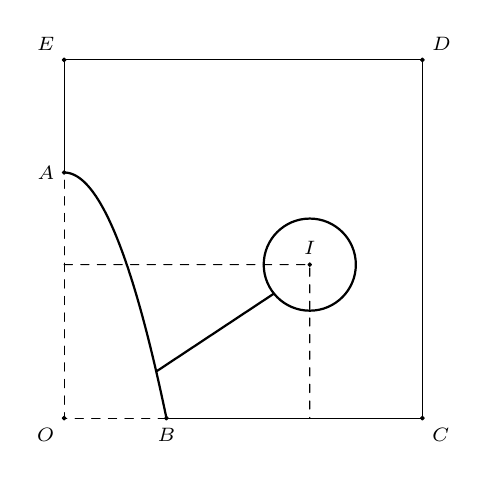
\begin{tikzpicture}[line join = round, line cap = round,>=stealth,font=\scriptsize,scale=0.65]
			%Bờ AB
			\draw[thick,smooth,samples=200,domain=0:2] plot (\x,{-6/5*((\x)^2)+0*\x+24/5});
			%Bờ AE ED DC CB
			\draw [dashed] (2,0)--(0,0)--(0,4.8);
			\draw (0,4.8)--(0,7)--(7,7)--(7,0)--(2,0);
			%Mảnh đất trồng rau
			\coordinate (I) at (4.8,3);
			\draw [thick] (I) circle(0.9);
			%Vẽ các điểm
			\draw [fill=black] (0,0)node[below left]{$O$}circle(1pt) (0,4.8)node[left]{$A$}circle(1pt) (0,7)node[above left]{$E$}circle(1pt) (7,7)node[above right]{$D$}circle(1pt) (7,0)node[below right]{$C$}circle(1pt) (2,0)node[below]{$B$}circle(1pt) (4.8,3)node[above]{$I$}circle(1pt);
			\draw [dashed] (0,3)--(I)--(4.8,0);
			%Vẽ cây cầu
			\draw [thick] (1.8,0.912)--(4.1,2.4343);
		\end{tikzpicture}
	}
	\shortans[oly]{$25,2$}
	\loigiai{
		Chọn hệ trục tọa độ $Oxy$ với gốc $O$, chiều dương trục hoành là tia $OC$, chiều dương trục tung là tia $OE$, đơn vị hai trục là {ex}vị độ dài (1 mét).\\
		Khi đó, ta có phương trình đường parabol là $y=-\dfrac3{25}x^2+48$ và p{ex}g trình đường tròn tâm $I(48; 30)$, bán kính $R=9$ là $(x-48)^2+(y-30)^2=81$.\\
		Xét điểm $M\left(a; -\dfrac{3}{25}a^2+48\right)$ với $0\le a\le 20$ nằm trên parabol thì khoảng cách từ đường tròn đến parabol là $d=MI-R=\sqrt{(48-a)^2+\left(-\dfrac3{25}a^2+48-30\right)^2}-9$.\\
		Khảo sát hàm số ta tìm được khoảng cách ngắn nhất xấp xỉ $25,2$ (mét).
	}
\end{ex}
%%%==============HetCau_EX1==============%%%
%%%==============Cau_EX2==============%%%
\begin{ex}%[Dự án C THPTQG 2025]%[ĐỖ CHÍ TÂM]	%[2H3K1-4]
	Hai chiếc máy bay không người lái cùng bay lên từ một địa điểm. Sau một giờ bay, chiếc thứ nhất cách điểm xuất phát về phía bắc $23$ km và về phía tây $18$ km, đồng thời cách mặt đất $2$ km. Chiếc thứ hai cách điểm xuất phát về phía đông $22$ km và về phía nam $27$ km, đồng thời cách mặt đất $3$ km. Chọn hệ trục tọa độ $Oxyz$ với gốc tọa độ $O$ đặt tại vị trí xuất của hai chiếc máy bay, mặt phẳng $Oxy$ trùng với mặt đất sao cho trục $Ox$ hướng về phía bắc, trục $Oy$ hướng về phía tây và trục $Oz$ hướng thẳng đứng lên trời, đơn vị đo lấy theo ki-lô-mét. Sau đúng một giờ bay, hai máy bay đó cùng bắn một mục tiêu di động trên mặt đất. Biết tổng khoảng cách từ mỗi máy bay đến mục tiêu là nhỏ nhất, lúc đó mục tiêu cách điểm xuất phát của hai máy bay bao nhiêu ki-lô-mét (kết quả làm tròn đến hàng phần trăm)?
	\par
	\shortans[oly]{$5$}
	\loigiai{
		Với hệ trục tọa độ được chọn. Sau một giờ bay, máy bay thứ nhất có vị trí là điểm $A(23; 18; 2)$, máy bay thứ hai có vị trí là điểm $B(-22; -27; 3)$.\\
		Gọi $M$ là vị trí của mục tiêu. Vì mục tiêu di chuyển trên mặt đất nên $M\in(Oxy)\Rightarrow M(a; b; 0)$.\\
		Ta cần tìm $M$ để $MA+MB$ nhỏ nhất.\\
		Ta có $A$, $B$ nằm cùng phía đối với mặt phẳng $(Oxy)$. Gọi $B'$ là điểm đối xứng với $B$ qua mặt phẳng $(Oxy)\Rightarrow B'(-22; -27; -3) $ và $MB=MB'$.\\
		Ta có $MA+MB=MA+MB'\ge AB'$.\\
		Suy ra $MA+MB$ nhỏ nhất bằng $AB'$ khi $M$ là giao điểm của $AB'$ với mặt phẳng $(Oxy)$ hay ba điểm $A$, $M$, $B'$ thẳng hàng.\\
		Ta có $\heva{&\vec{AM}=(a-23; b-18; -2)\\&\vec{AB'}=(-45; -45; -5)}$.\\
		Ba điểm $A$, $M$, $B'$ thẳng hàng khi chỉ khi $\dfrac{a-23}{-45}=\dfrac{b-18}{-45}=\dfrac{-2}{-5}\Leftrightarrow\heva{&a=5\\&b=0}\Rightarrow M(5; 0; 0)$.\\
		Vậy khoảng cách từ mục tiêu đến vị trí xuất phát ban đầu của máy bay là đoạn $$OA=\sqrt{(5-0)^2+(0-0)^2+(0-0)^2}=5\text{ km}.$$
	}
\end{ex}
%%%==============HetCau_EX2==============%%%
%%%==============Cau_EX3==============%%%
\begin{ex}%[Dự án C THPTQG 2025]%[ĐỖ CHÍ TÂM]	%[1H8V5-3]
	Cho hình chóp $S.ABCD$ có đáy $ABCD$ là hình thoi tâm $O$, cạnh $AB=7$ và $\widehat{BAD}=120^\circ$, $SO\perp (ABCD)$ và $SO=7$. Tính khoảng cách từ điểm $O$ đến mặt phẳng $(SBC)$. (Kết quả làm tròn đến hàng phần mười).
	\par
	\shortans[oly]{$2,8$}
	\loigiai{
		\immini{
			Kẻ $OH\perp BC$ tại $H$. Kẻ $OK\perp HS$ tại $K$. Khi đó $\mathrm{d}(O,(SBC))=OK$.\\
			Vì $ABCD$ là hình thoi tâm $O$ cạnh bằng $7$ và có $\widehat{BAD}=120^\circ$, do đó $BO=\dfrac{7\sqrt2}{2}$, $OC=\dfrac72$; $BC=7$.\\
			Xét tam giác $OBC$ vuông tại $O$ có $OH$ là đường cao nên $OH=\dfrac{BO\cdot OC}{BC}=\dfrac{7\sqrt3}{4}$.\\
			Xét tam giác $SOH$ vuông tại $O$ có đường cao $OK$ nên $OK=\dfrac{OS\cdot OH}{OS^2+OH^2}=\dfrac{7\sqrt{57}}{19}\approx 2{,}8$.\\
			Vậy khoảng cách từ điểm $O$ đến mặt phẳng $(SBC)$ xấp xỉ bằng $2{,}8$.
		}{
 \begin{tikzpicture}[thick, scale=0.7]
  %%\draw[gray!20] (-3,-2) grid (6,5);
  \path (0,0) coordinate (A)  
  (-2,-2) coordinate (D)
  (5,0) coordinate (B)
  (3,-2) coordinate (C)
  (3/2,4) coordinate (S)
  (3/2, -1) coordinate (O);
  \path ($(B)!0.6!(C)$) coordinate (H)
        ($(S)!0.7!(H)$) coordinate (K);
  \draw[dashed] (S)-- (A)--(D) (A)--(B) (O)--(S) (A)--(C) (D)--(B) (O)--(K) (O)--(H);
  \draw (D)--(C)--(B)--(S)--(D) (S)--(C) (S)--(H);
  \foreach \p/\q in {A/180, D/-90, C/-90, B/0, S/90, O/-90, H/-90, K/45}
  \fill[blue] (\p) circle(2pt) node[shift={(\q:3mm)}]{\bfseries $\p$};
  	\path pic[draw,angle radius=5pt]{right angle= O--H--C};
  	\path pic[draw,angle radius=5pt]{right angle= O--K--H};
 \end{tikzpicture}			
		}
	}
\end{ex}
%%%==============HetCau_EX3==============%%%
%%%==============Cau_EX4==============%%%
\begin{ex}%[Dự án C THPTQG 2025]%[ĐỖ CHÍ TÂM]%[2D1K3-6]	
	Công ty $A$ dự định tổ chức cho nhân viên đi tham quan Huế trong hai ngày. Công ty $A$ dự định nếu đặt giá tua của công ty du lịch $B$ là $2{,}1$ triệu đồng một người thì sẽ có khoảng $142$ người tham gia. Để kích thích mọi người tham gia, công ty du lịch $B$ quyết định giảm giá và cứ mỗi lần giảm giá tua $100$ nghìn đồng thì sẽ có thêm $20$ người tham gia. Hỏi công ty du lịch $B$ phải bán giá tua là bao nhiêu triệu đồng một người để doanh thu từ tua là lớn nhất (kết quả làm tròn đến hàng phần trăm)?
	\par
	\shortans[oly]{$1,41$}
	\loigiai{
		Gọi số lần giảm $100$ nghìn đồng là $x$ ($x>0$).\\
		Giá tham gia tua của một người là $2{,}1-0{,}1x$ (triệu đồng/người).\\
		Số người tham gia tua là $142+20x$ (người).\\
		Doanh thu $f(x)=(2{,}1-0{,}1x)(142+20x)=-2x^2+27{,}8x+298{,}2$.\\
		Do $f(x)$ là đa thức bậc hai có hệ số $a<0$ nên $f(x)$ đạt giá trị lớn nhất tại $x=\dfrac{-27{,}8}{2\cdot(-2)}=6{,}95$.\\
		Vậy giá vé tham gia tua của một người để doanh thu lớn nhất là $$2{,}1-0{,}1\cdot6{,}95=1{,}41\text{ (triệu đồng)}$$
	}
\end{ex}
%%%==============HetCau_EX4==============%%%
%%%==============Cau_EX5==============%%%
\begin{ex}%[Dự án C THPTQG 2025]%[ĐỖ CHÍ TÂM]	%[1C2V3-1]
	\immini{
		Một người khách nước ngoài sang Việt Nam dự định thuê ô-tô đi du lịch bằng cách lựa chọn xuất phát từ một tỉnh bất kỳ trong các tỉnh $A$, $B$, $C$, $D$, $E$ và lần lượt đi qua các tỉnh còn lại (mỗi tỉnh đi qua một lần duy nhất) rồi quay trở về tỉnh ban đầu với thời gian (đơn vị là giờ) đi giữa các tỉnh được cho như hình vẽ. Biết giá thuê xe ở thời điểm hiện tại là $50\,000$ đồng/giờ và không thay đổi trong suốt hành trình. Hỏi chi phí tiền thuê xe ít nhất bằng bao nhiêu triệu đồng để người đó có thể thể hoàn thành chuyến đi của mình?
	}{
		\begin{tikzpicture}[line join = round, line cap = round,>=stealth,font=\scriptsize,scale=0.65]
			\coordinate (A) at (-2,4.5);
			\coordinate (B) at (-2,1);
			\coordinate (C) at (-4,-2);
			\coordinate (D) at (4,-2);
			\coordinate (E) at (0,0);
			
			\coordinate (m) at ($(A)!0.5!(B)$);
			\coordinate (n) at ($(B)!0.5!(C)$);
			\coordinate (p) at ($(C)!0.5!(D)$);
			\coordinate (q) at ($(A)!0.5!(D)$);
			\coordinate (r) at ($(A)!0.5!(E)$);
			\coordinate (s) at ($(B)!0.5!(E)$);
			\coordinate (t) at ($(C)!0.5!(E)$);
			\coordinate (u) at ($(E)!0.5!(D)$);
			
			\draw (A)--(B)--(C)--(D)--(A)--(E)--(D) (B)--(E)--(C);
			\draw [fill=white] (A)circle(0.35)node{$A$} (B)circle(0.35)node{$B$} (C)circle(0.35)node{$C$} (D)circle(0.35)node{$D$} (E)circle(0.35)node{$E$};
			
			\draw (m)node[left]{$17$} (n)node[left]{$12$} (p)node[below]{$10$} (q)node[above]{$20$} (r)node[right]{$8$} (s)node[above]{$29$} (t)node[above]{$19$} (u)node[above]{$9$};
		\end{tikzpicture}
	}
	\par
	\shortans[oly]{$2,8$}
	\loigiai{
		Giả sử người đi du lịch xuất phát từ tỉnh $A$.\\
		Hành trình ngắn nhất người đó có thể đi là $A\to B\to C\to D\to E\to A$.\\
		Thời gian để xe di chuyển là $17+12+10+9+8=56$.\\
		Chi phí cần chi trả là $56\cdot 50\,000=2\,800\,000$ đồng.\\
		Vậy chi phí thấp nhất để người đó hoàn thành chuyến du lịch là $2{,}8$ triệu đồng.
	}
\end{ex}
%%%==============HetCau_EX5==============%%%
%%%==============Cau_EX6==============%%%
\begin{ex}%[Dự án C THPTQG 2025]%[ĐỖ CHÍ TÂM]%[0D0C2-4]
	Nhân dịp Tết Trung thu cô giáo tặng quà cho ba bạn Vũ, Hồng, Ngọc. Trong hộp quà có $9$ cây bút và $8$ quyển vở được để một cách lộn xộn. Cô giá gọi ba bạn xếp hàng theo thứ tự: Vũ đứng trước nhận quà đầu tiên, Hồng đứng sau Vũ nên được nhận quà thứ hai, Ngọc đứng sau cùng nên nhận quà sau cùng. Xác suất để Ngọc nhận quà là cây bút bằng bao nhiêu, biết rằng cô giáo tặng quà bằng cách rút ngẫu nhiên và mỗi bạn chỉ nhận một phần quà trong hộp (kết quả làm tròn đến hàng phần trăm)?
	\par
	\shortans[oly]{$0,53$}
	\loigiai{
		Ta xét các trường hợp sau
		\begin{itemize}
			\item \textbf{Trường hợp 1:} Vũ nhận bút, Hồng nhận bút, Ngọc nhận bút.\\
			Xác suất Vũ nhận bút là $\dfrac9{17}$.\\
			Xác suất Hồng nhận bút là $\dfrac{8}{16}=\dfrac12$.\\
			Xác suất Ngọc nhận bút là $\dfrac{7}{15}$.\\
			Xác suất của trường hợp này là $\dfrac{9}{17}\cdot\dfrac{1}{2}\dfrac{7}{15}=\dfrac{63}{510}$.
			\item \textbf{Trường hợp 2:} Vũ nhận bút, Hồng nhận vở, Ngọc nhận bút.\\
			Xác suất Vũ nhận bút là $\dfrac9{17}$.\\
			Xác suất Hồng nhận vở là $\dfrac{8}{16}=\dfrac12$.\\
			Xác suất Ngọc nhận bút là $\dfrac{8}{15}$.\\
			Xác suất của trường hợp này là $\dfrac{9}{17}\cdot\dfrac{1}{2}\dfrac{8}{15}=\dfrac{72}{510}$.
			\item \textbf{Trường hợp 3:} Vũ nhận vở, Hồng nhận bút, Ngọc nhận bút.\\
			Xác suất Vũ nhận bút là $\dfrac8{17}$.\\
			Xác suất Hồng nhận vở là $\dfrac{9}{16}$.\\
			Xác suất Ngọc nhận bút là $\dfrac{8}{15}$.\\
			Xác suất của trường hợp này là $\dfrac{8}{17}\cdot\dfrac{9}{16}\dfrac{8}{15}=\dfrac{72}{510}$.
			\item \textbf{Trường hợp 4:} Vũ nhận vở, Hồng nhận vở, Ngọc nhận bút.\\
			Xác suất Vũ nhận bút là $\dfrac8{17}$.\\
			Xác suất Hồng nhận vở là $\dfrac{7}{16}$.\\
			Xác suất Ngọc nhận bút là $\dfrac{9}{15}$.\\
			Xác suất của trường hợp này là $\dfrac{8}{17}\cdot\dfrac{7}{16}\dfrac{9}{15}=\dfrac{63}{510}$.
		\end{itemize}
		Vậy xác suất để Ngọc nhận được bút là $$\dfrac{63}{510}+\dfrac{72}{510}+\dfrac{72}{510}+\dfrac{63}{510}=\dfrac{9}{17}\approx 0{,}53.$$
	}
\end{ex}
%%%==============HetCau_EX6==============%%%
 \Closesolutionfile{ans}
 \inputansbox{6,4,3}{ans/TT-THPT-SGD-TuyenQuang-NH24-25}